\pgfdeclarelayer{pic1}
\pgfdeclarelayer{ar1}
\pgfdeclarelayer{pic2}
\pgfdeclarelayer{ar2}
\pgfdeclarelayer{pic3}
\pgfdeclarelayer{ar3}
\pgfdeclarelayer{pic4}
\pgfdeclarelayer{ar4}                %
\pgfsetlayers{main,ar4,pic4,ar3,pic3,ar2,pic2,ar1,pic1}   




\newcommand{\hierarchy}[1]{
\begin{framet}{w}{Images/XDF.jpg}{

#1

\node (e) at (1,0.2) {};
%
\begin{pgfonlayer}{ar1}
\draw[-,DarkGrey] (a.south west) -- ([xshift=-25pt]b.center);
\draw[-,DarkGrey] (a.south east) -- ([xshift=-25pt]b.center);
\draw[-,DarkGrey] (a.north west) -- ([xshift=-25pt]b.center);
\draw[-,DarkGrey] (a.north east) -- ([xshift=-25pt]b.center);
\end{pgfonlayer}
%
\begin{pgfonlayer}{ar2}
\draw[-,DarkGrey] (b.south west) -- ([xshift=40pt,yshift=-20pt]c.center);
\draw[-,DarkGrey] (b.south east) -- ([xshift=40pt,yshift=-20pt]c.center);
\draw[-,DarkGrey] (b.north west) -- ([xshift=40pt,yshift=-20pt]c.center);
\draw[-,DarkGrey] (b.north east) -- ([xshift=40pt,yshift=-20pt]c.center);
\end{pgfonlayer}
%
\begin{pgfonlayer}{ar3}
\draw[-,DarkGrey] (c.south west) -- ([xshift=22pt,yshift=-18pt]d.center);
\draw[-,DarkGrey] (c.south east) -- ([xshift=22pt,yshift=-18pt]d.center);
\draw[-,DarkGrey] (c.north west) -- ([xshift=22pt,yshift=-18pt]d.center);
\draw[-,DarkGrey] (c.north east) -- ([xshift=22pt,yshift=-18pt]d.center);
\end{pgfonlayer}
%
\begin{pgfonlayer}{ar4}
\draw[-,DarkGrey] (d.south west) -- (e.center);
\draw[-,DarkGrey] (d.south east) -- (e.center);
\draw[-,DarkGrey] (d.north west) -- (e.center);
\draw[-,DarkGrey] (d.north east) -- (e.center);
\end{pgfonlayer}


}
\frametitle{Our Picture of the Universe}
\end{framet}
}

\newcommand{\hierarchyblank}{
\hierarchy{
\begin{pgfonlayer}{pic1}
\node[inner sep=0.5pt] (a) at (1.1,2.1)[draw=DarkGrey] {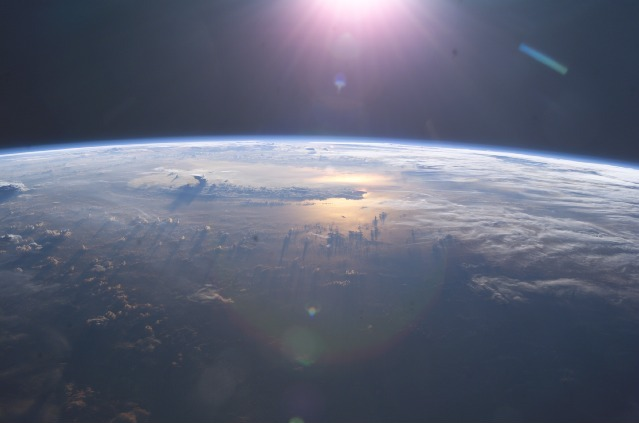
\includegraphics[width=0.35\paperwidth]{Images/Earth.jpg}};
\end{pgfonlayer}
%
\begin{pgfonlayer}{pic2}
\node[inner sep=0.5pt] (b) at (2.9,2.1)[draw=DarkGrey] {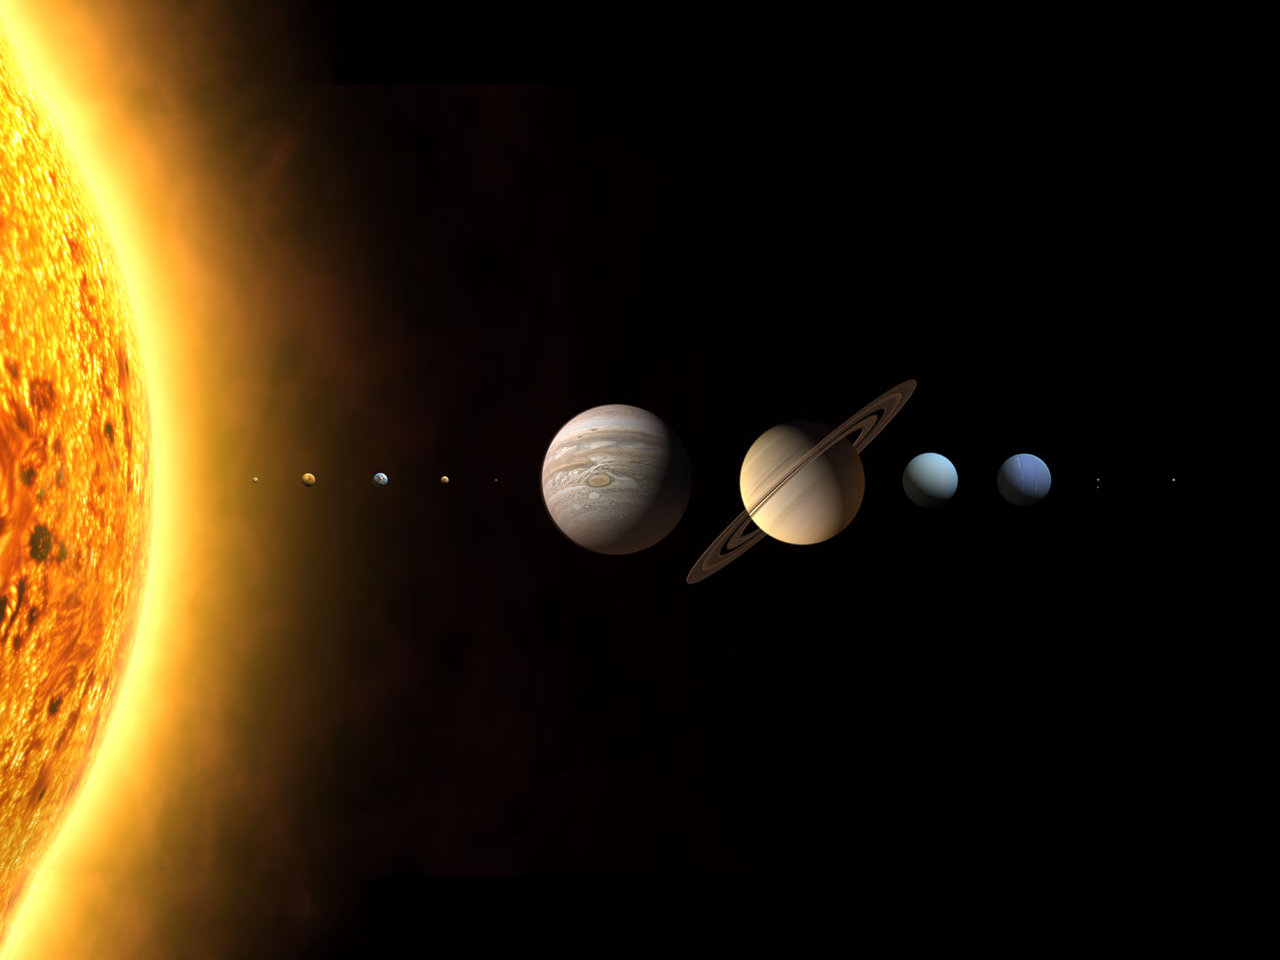
\includegraphics[width=0.35\paperwidth]{Images/solar_system1.jpg}};
\end{pgfonlayer}
%
\begin{pgfonlayer}{pic3}
\node[inner sep=0.5pt] (c) at (2.9,0.9)[draw=DarkGrey] {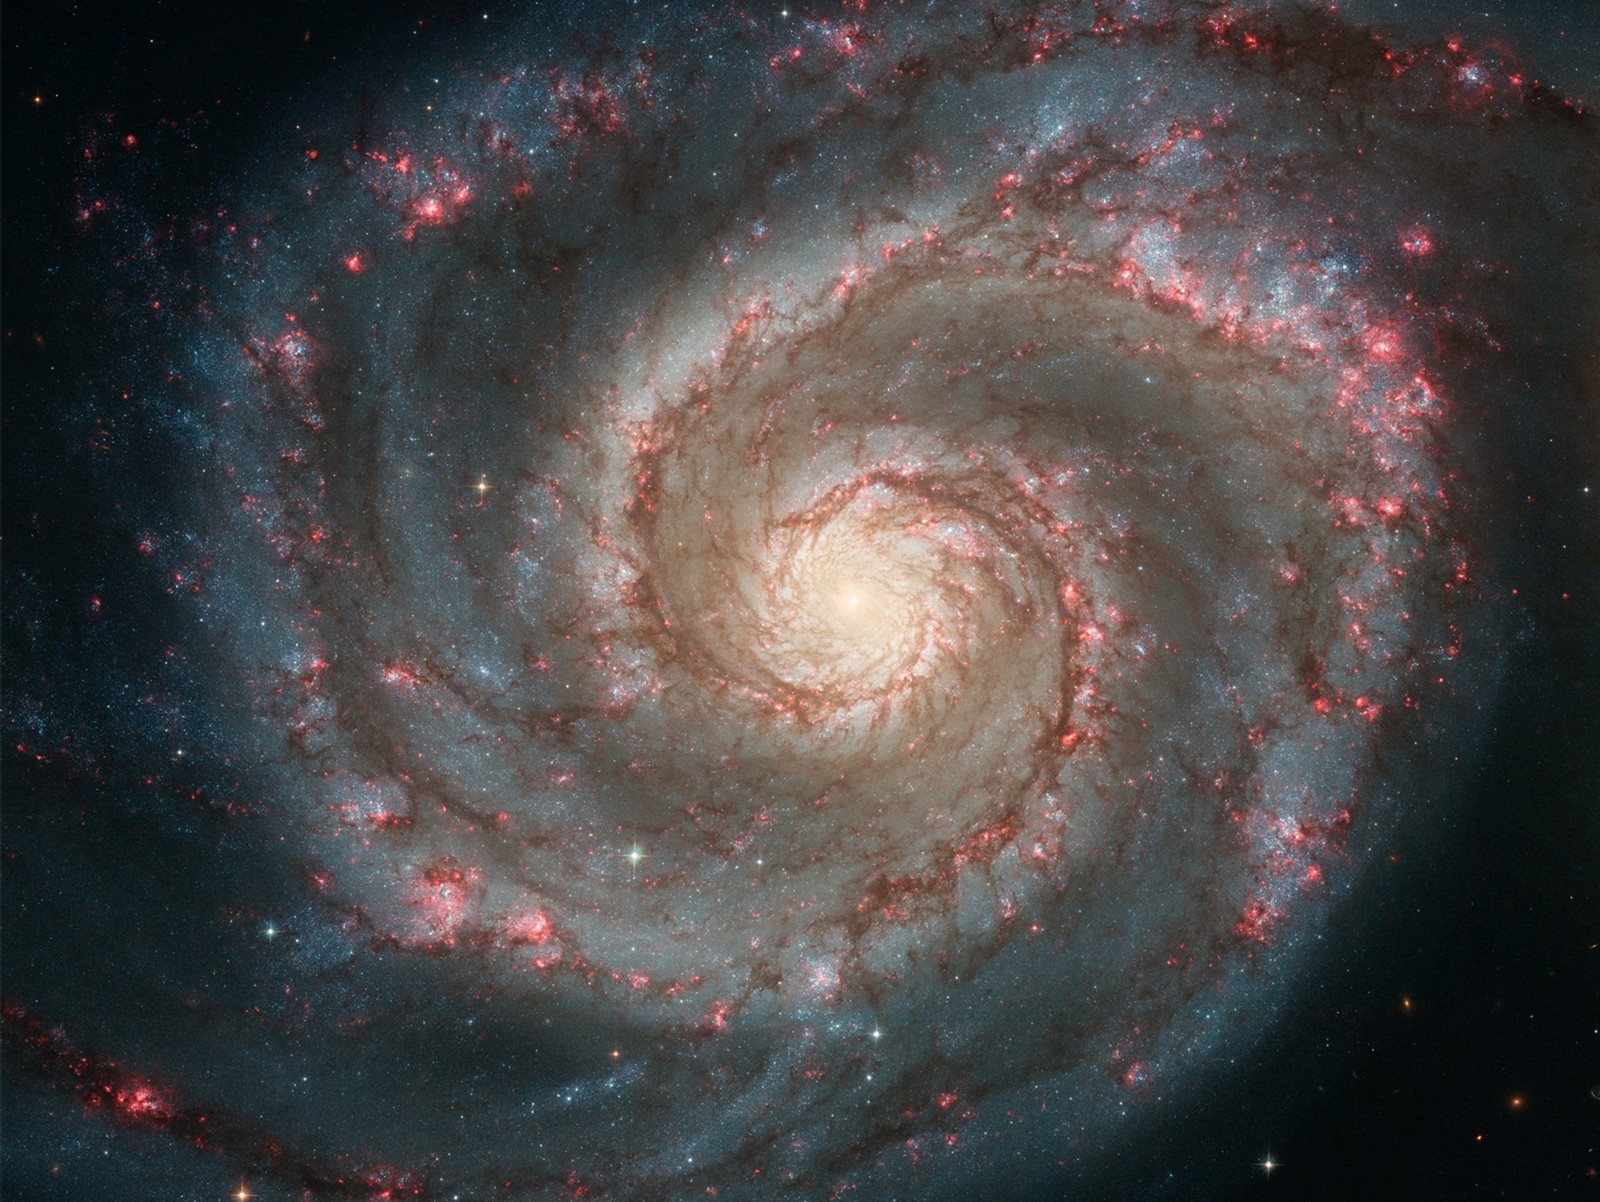
\includegraphics[width=0.35\paperwidth]{Images/milky_way.jpg}};
\end{pgfonlayer}
%
\begin{pgfonlayer}{pic4}
\node[inner sep=0.5pt] (d) at (1.1,0.9)[draw=DarkGrey] {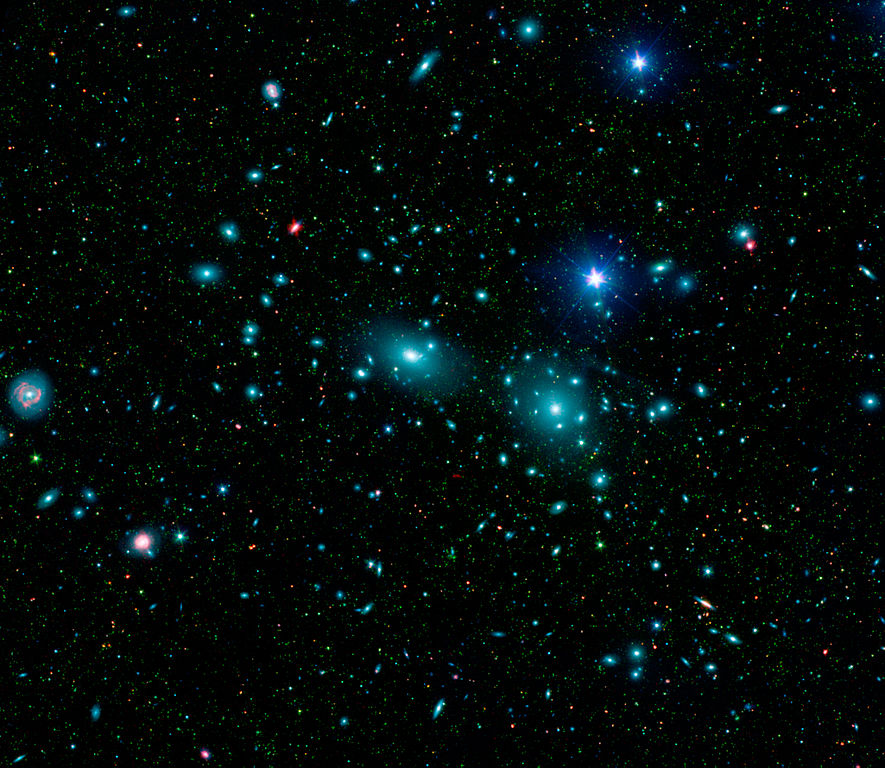
\includegraphics[width=0.35\paperwidth]{Images/Coma.jpg}};
\end{pgfonlayer}
}
}

\hierarchyblank

\hierarchy{
\begin{pgfonlayer}{pic1}
\node[inner sep=0.5pt] (a) at (1.1,2.1)[draw=red] {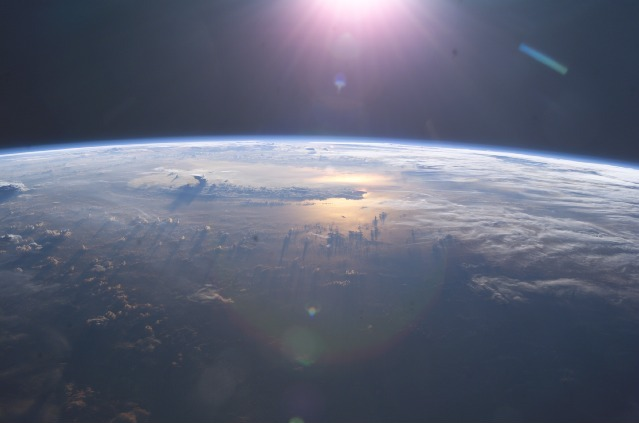
\includegraphics[width=0.35\paperwidth]{Images/Earth.jpg}};
\end{pgfonlayer}
%
\begin{pgfonlayer}{pic2}
\node[inner sep=0.5pt] (b) at (2.9,2.1)[draw=DarkGrey] {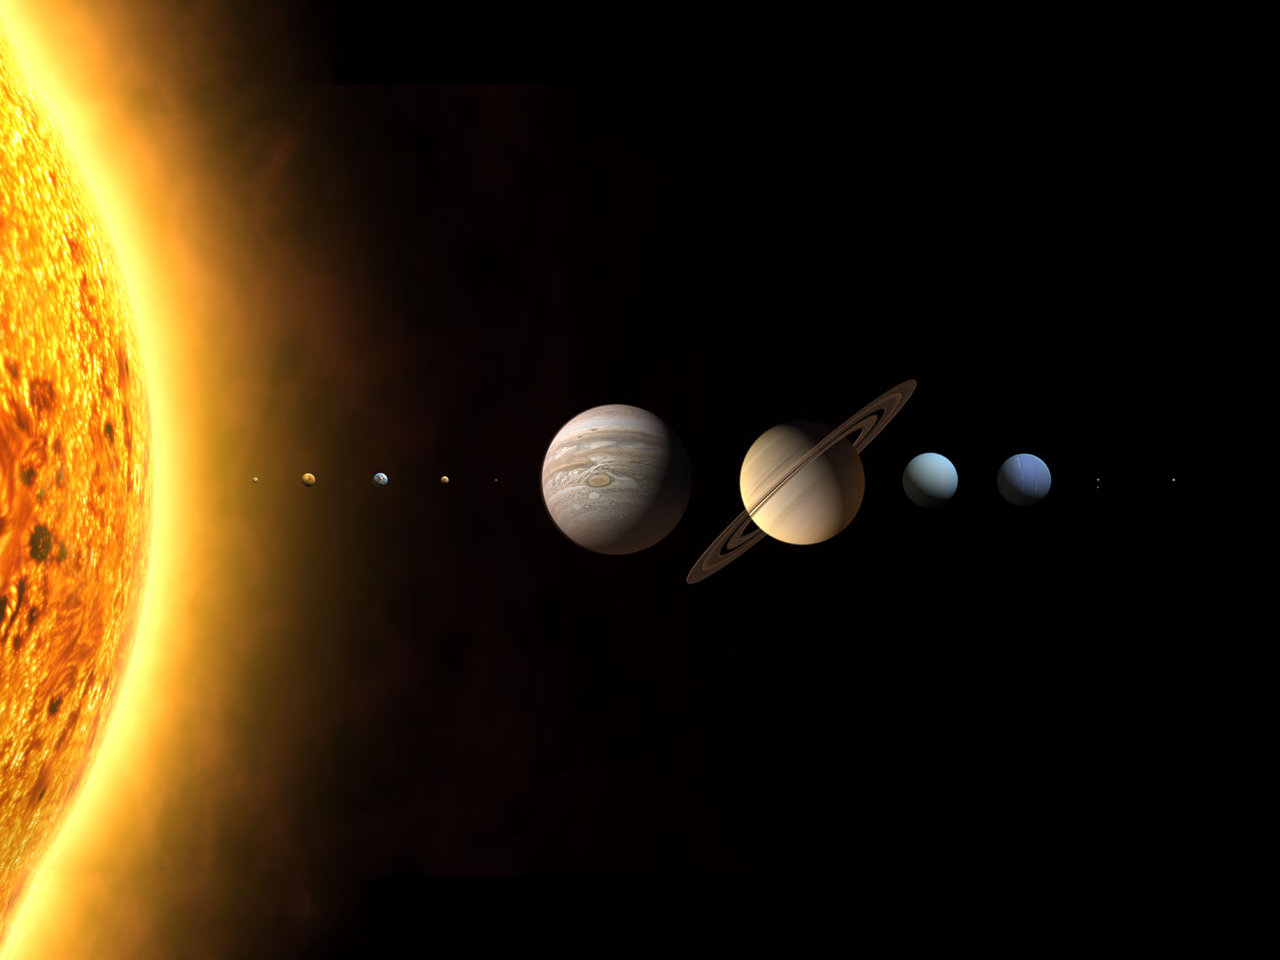
\includegraphics[width=0.35\paperwidth]{Images/solar_system1.jpg}};
\end{pgfonlayer}
%
\begin{pgfonlayer}{pic3}
\node[inner sep=0.5pt] (c) at (2.9,0.9)[draw=DarkGrey] {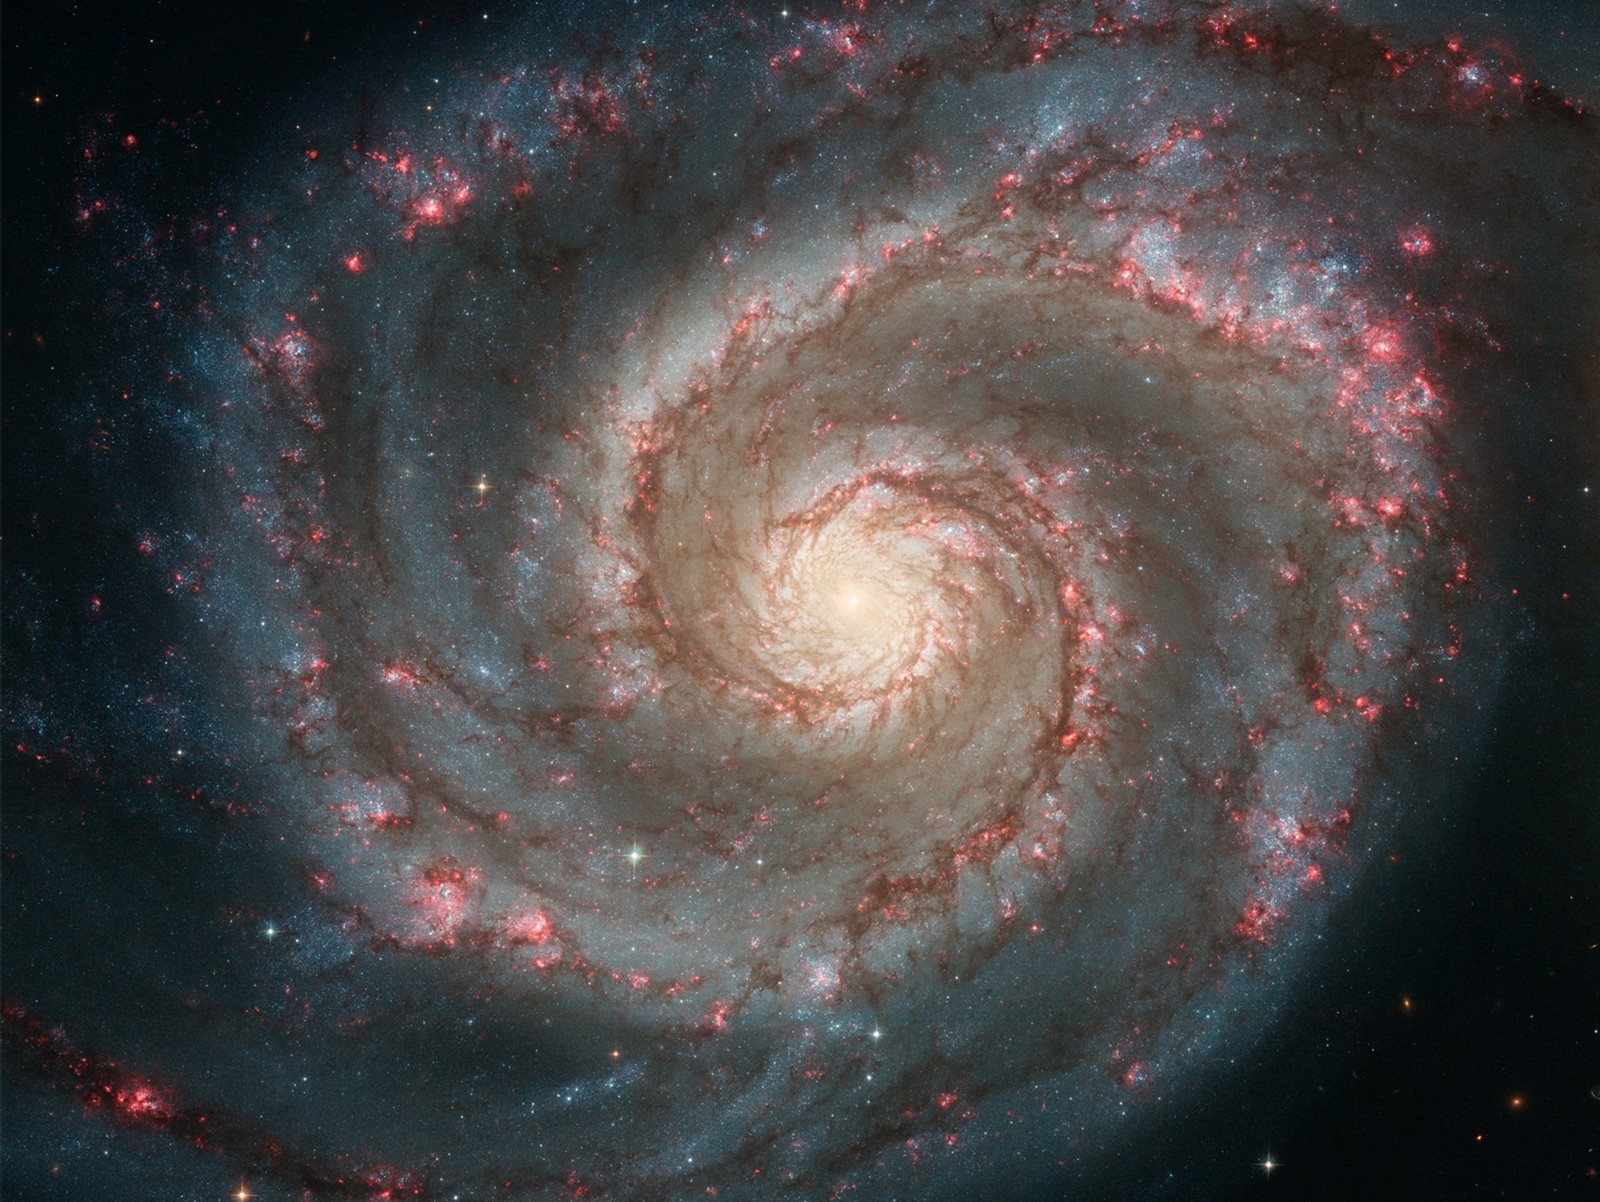
\includegraphics[width=0.35\paperwidth]{Images/milky_way.jpg}};
\end{pgfonlayer}
%
\begin{pgfonlayer}{pic4}
\node[inner sep=0.5pt] (d) at (1.1,0.9)[draw=DarkGrey] {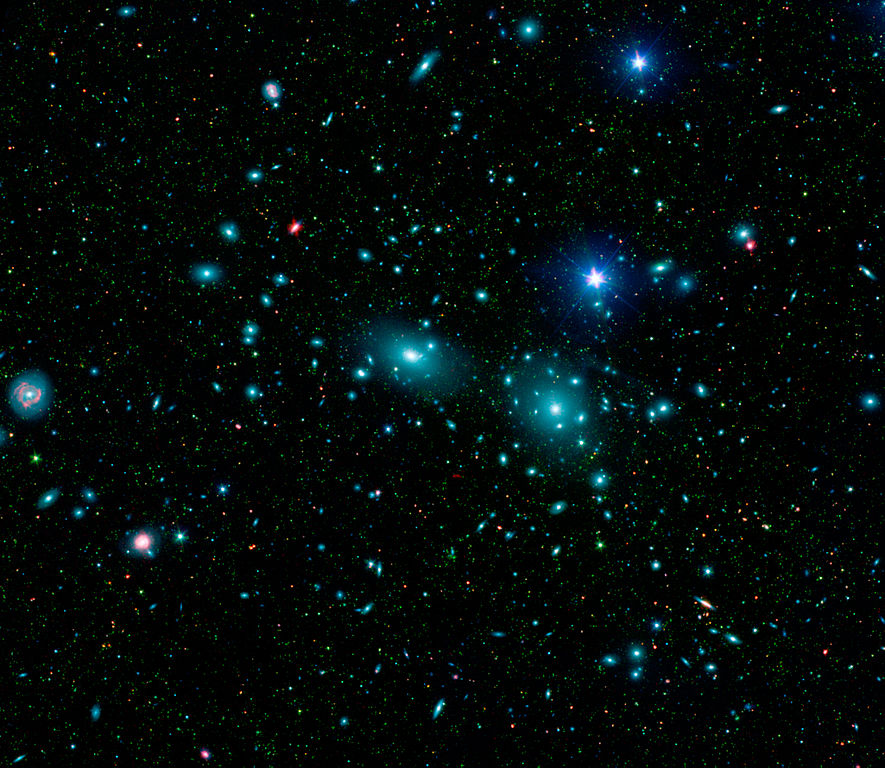
\includegraphics[width=0.35\paperwidth]{Images/Coma.jpg}};
\end{pgfonlayer}
}

\begin{frameb}{h}{Images/Earth.jpg}
	\frametitle{Earth}
\end{frameb}

\hierarchyblank
\hierarchy{
\begin{pgfonlayer}{pic1}
\node[inner sep=0.5pt] (a) at (1.1,2.1)[draw=DarkGrey] {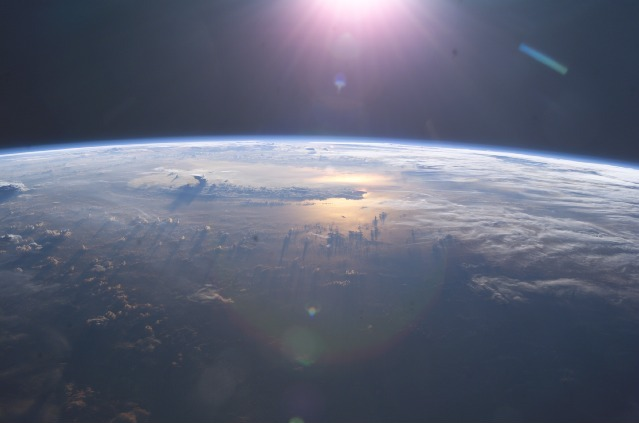
\includegraphics[width=0.35\paperwidth]{Images/Earth.jpg}};
\end{pgfonlayer}
%
\begin{pgfonlayer}{pic2}
\node[inner sep=0.5pt] (b) at (2.9,2.1)[draw=red] {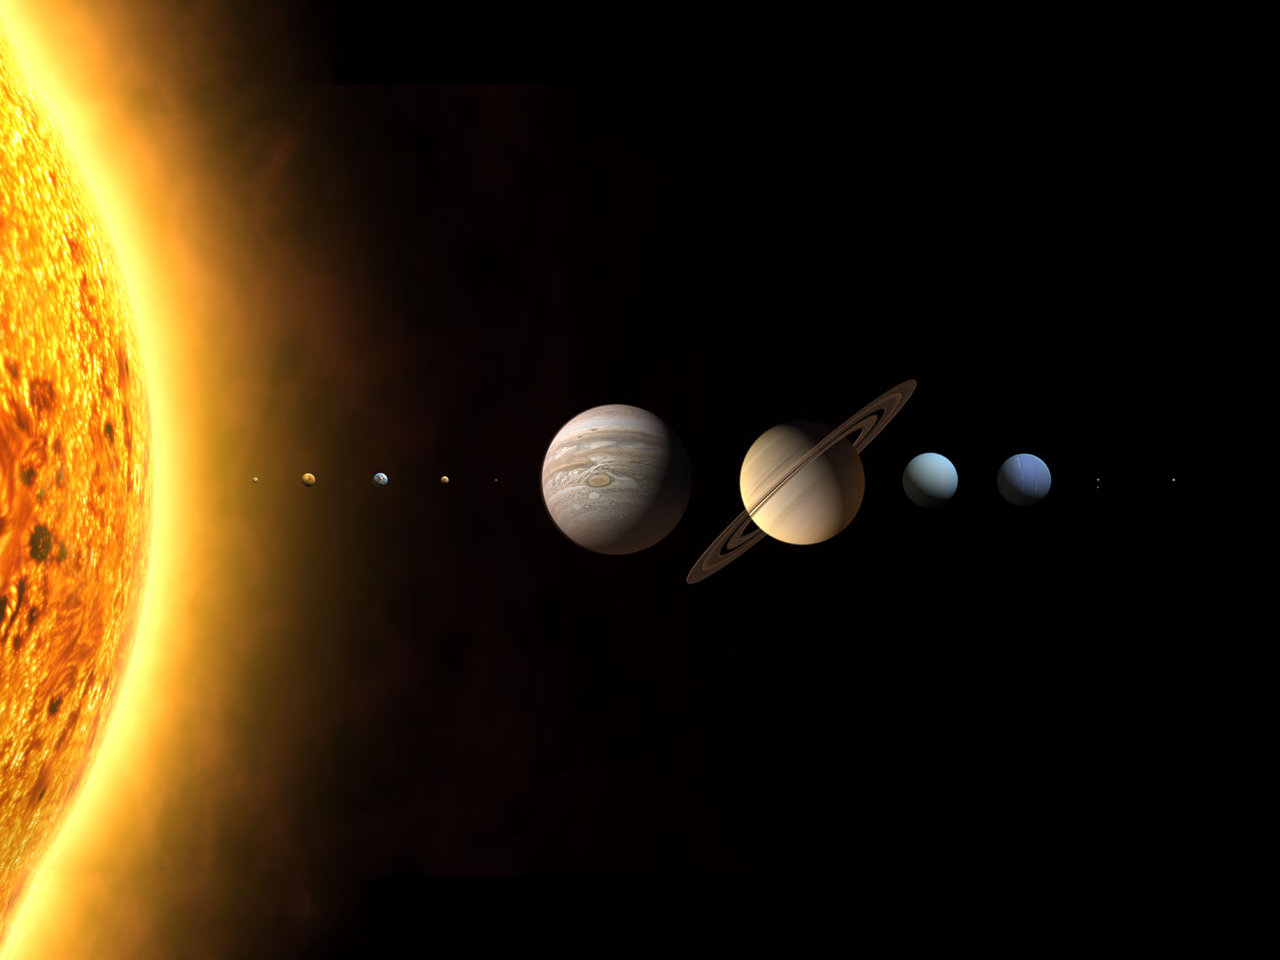
\includegraphics[width=0.35\paperwidth]{Images/solar_system1.jpg}};
\end{pgfonlayer}
%
\begin{pgfonlayer}{pic3}
\node[inner sep=0.5pt] (c) at (2.9,0.9)[draw=DarkGrey] {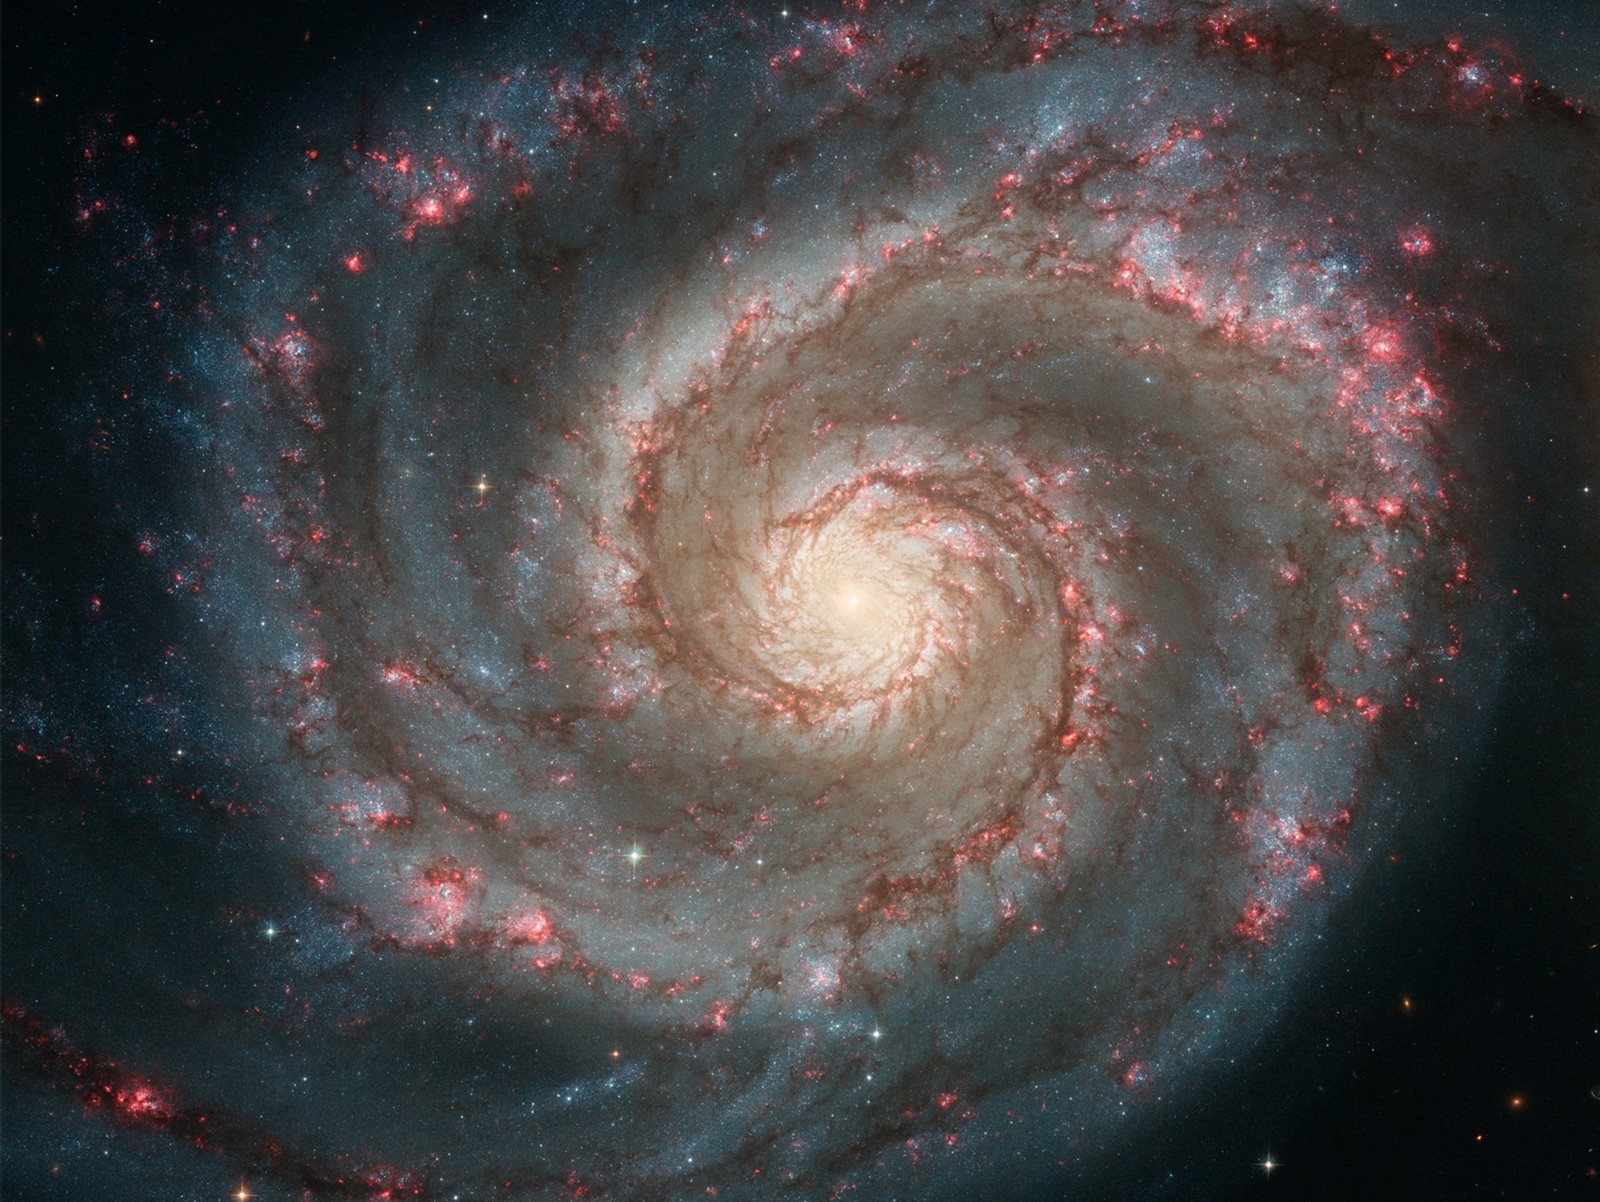
\includegraphics[width=0.35\paperwidth]{Images/milky_way.jpg}};
\end{pgfonlayer}
%
\begin{pgfonlayer}{pic4}
\node[inner sep=0.5pt] (d) at (1.1,0.9)[draw=DarkGrey] {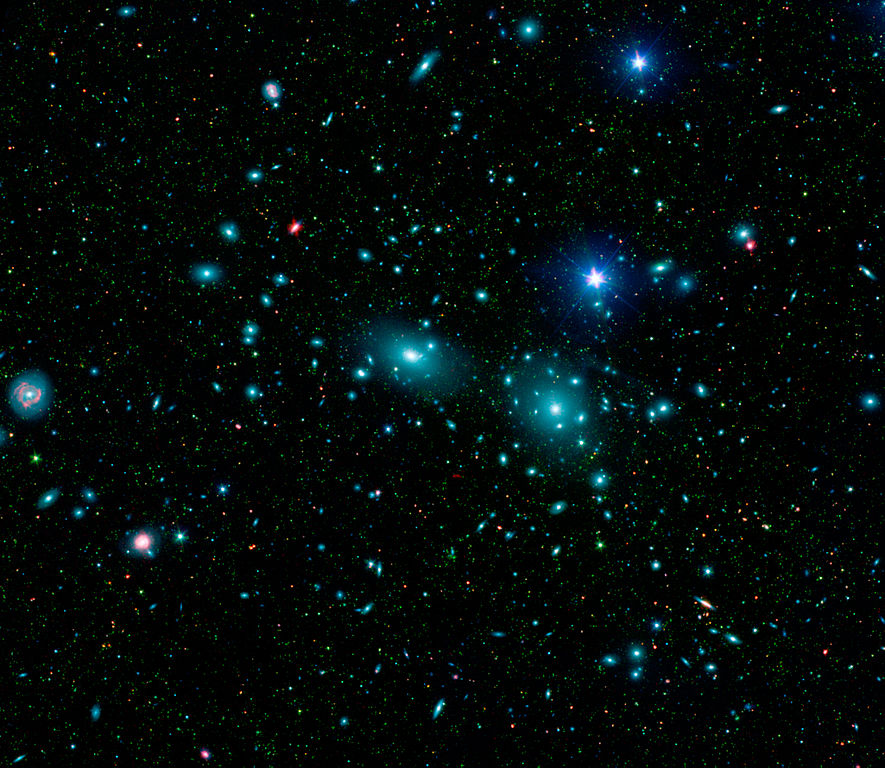
\includegraphics[width=0.35\paperwidth]{Images/Coma.jpg}};
\end{pgfonlayer}
}

\begin{frameb}{w}{Images/solar_system1.jpg}
	\frametitle{The Solar System}
	\begin{textblock}{20}(12,3)
	$\sim50$ AU
	\end{textblock}
	\begin{textblock}{30}(3,3)
	$1$ AU $\sim 8$ light minutes
	\end{textblock}
\end{frameb}


\hierarchyblank
\hierarchy{
\begin{pgfonlayer}{pic1}
\node[inner sep=0.5pt] (a) at (1.1,2.1)[draw=DarkGrey] {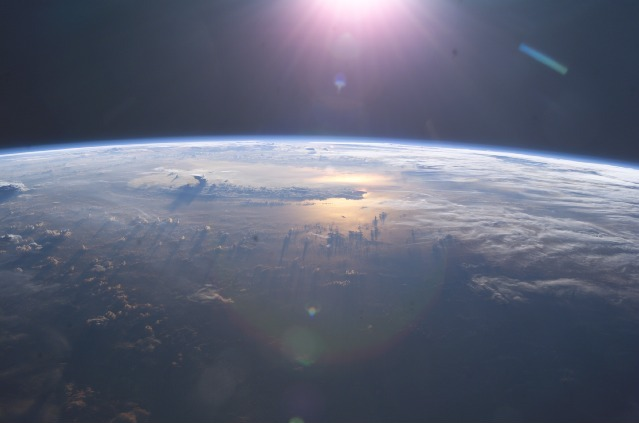
\includegraphics[width=0.35\paperwidth]{Images/Earth.jpg}};
\end{pgfonlayer}
%
\begin{pgfonlayer}{pic2}
\node[inner sep=0.5pt] (b) at (2.9,2.1)[draw=DarkGrey] {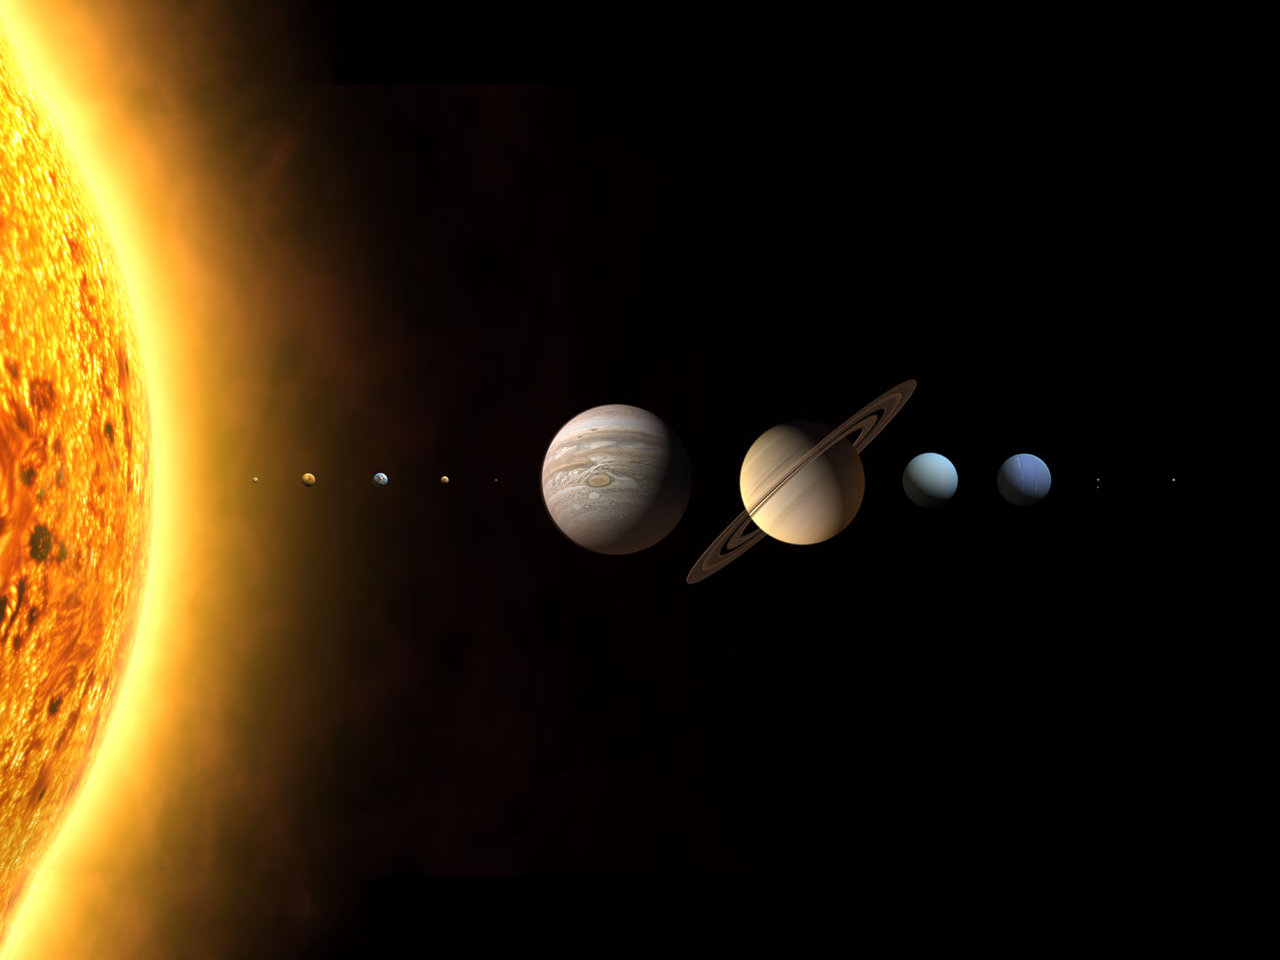
\includegraphics[width=0.35\paperwidth]{Images/solar_system1.jpg}};
\end{pgfonlayer}
%
\begin{pgfonlayer}{pic3}
\node[inner sep=0.5pt] (c) at (2.9,0.9)[draw=red] {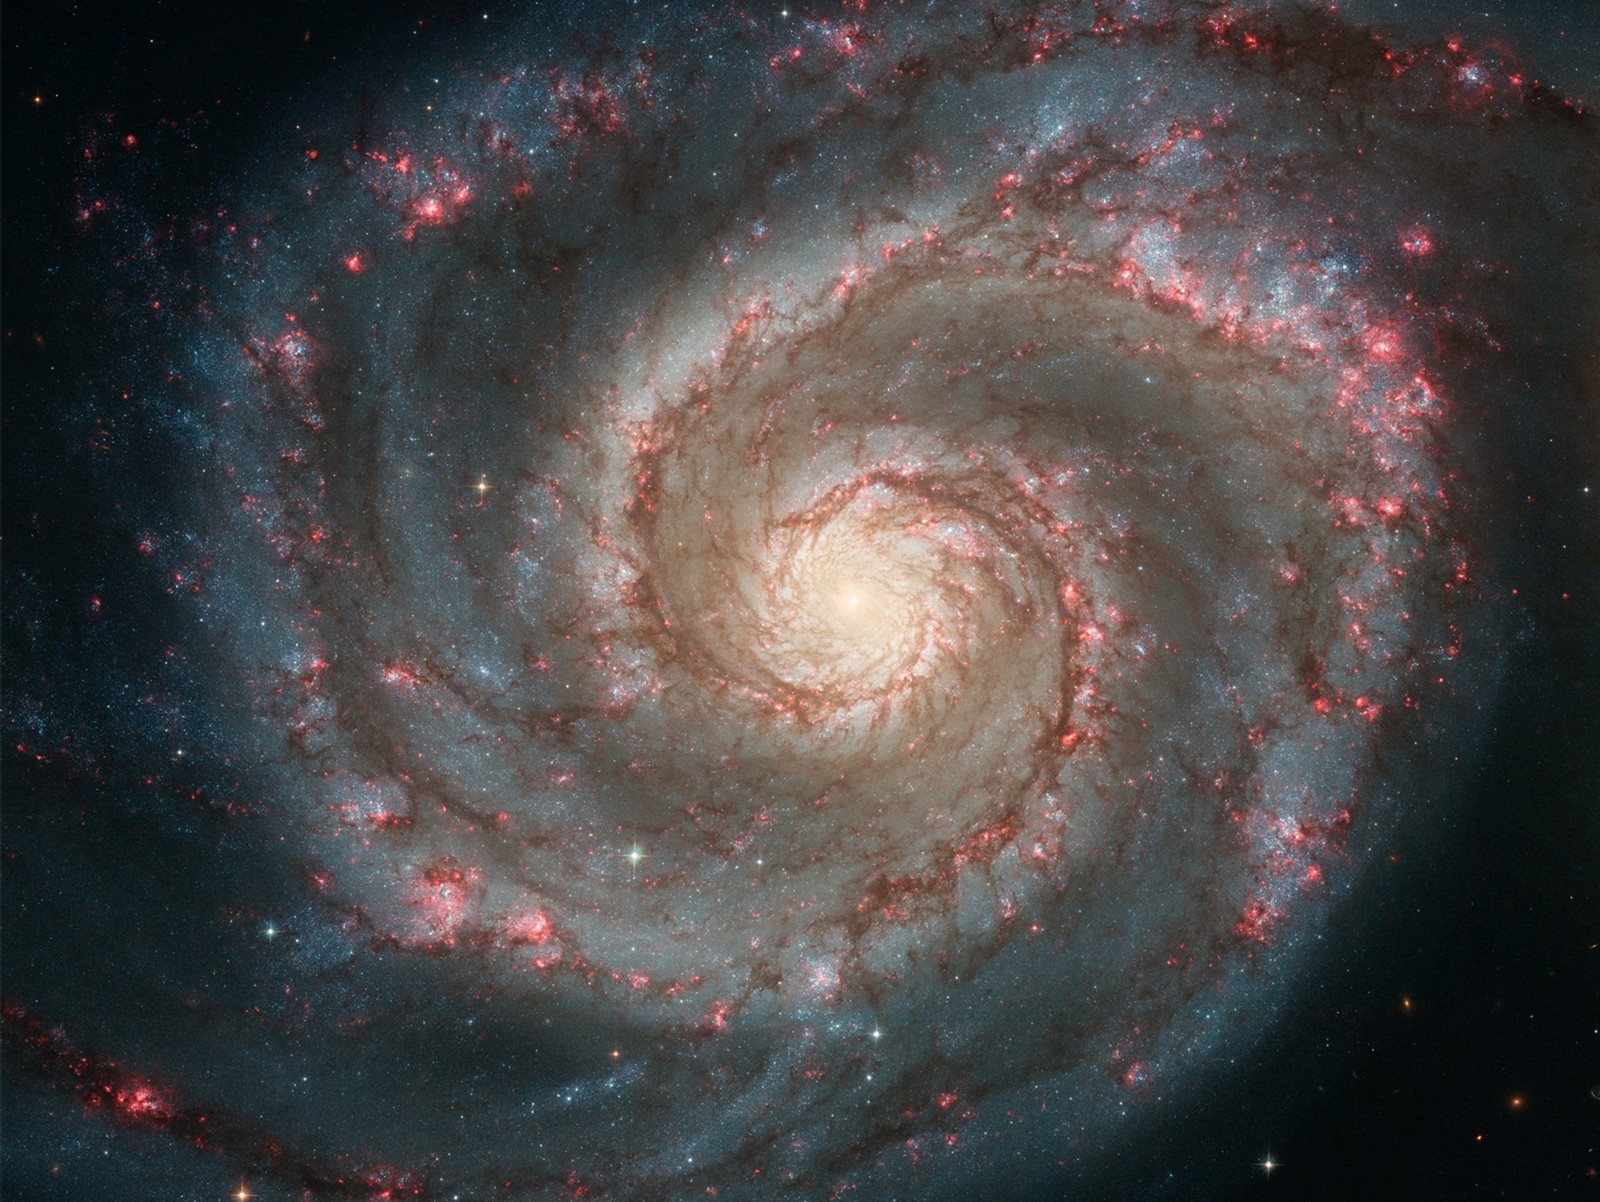
\includegraphics[width=0.35\paperwidth]{Images/milky_way.jpg}};
\end{pgfonlayer}
%
\begin{pgfonlayer}{pic4}
\node[inner sep=0.5pt] (d) at (1.1,0.9)[draw=DarkGrey] {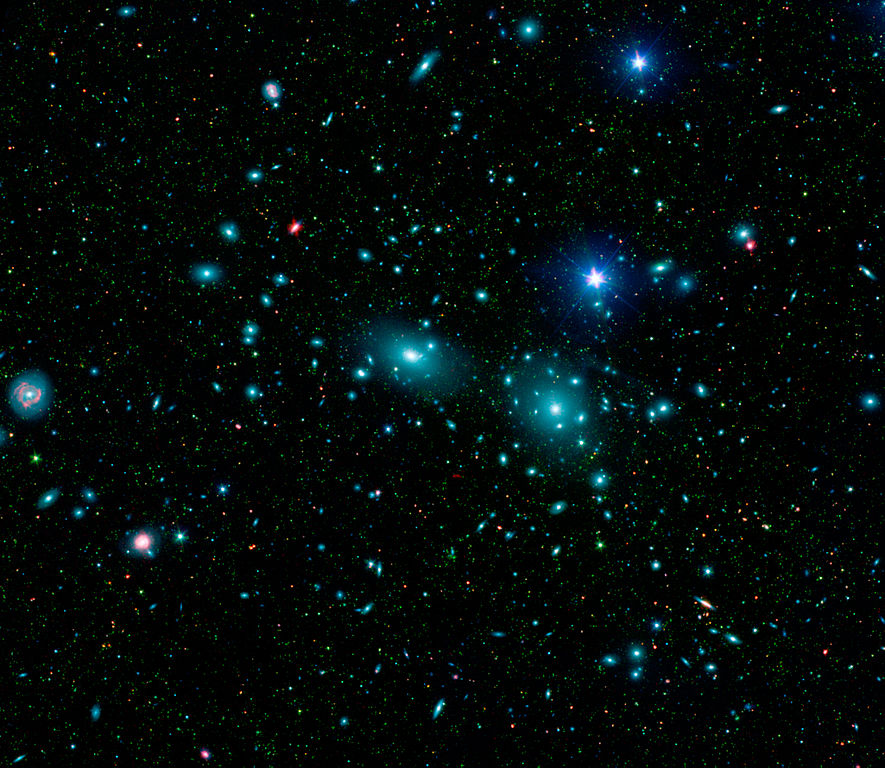
\includegraphics[width=0.35\paperwidth]{Images/Coma.jpg}};
\end{pgfonlayer}
}


\begin{frameb}{w}{Images/milky_way.jpg}
	\frametitle{Galaxies}
	\begin{textblock}{20}(8,7)
	$\sim 30$ kpc $\sim 100,000$ light years
	\end{textblock}
\end{frameb}



\hierarchyblank
\hierarchy{
\begin{pgfonlayer}{pic1}
\node[inner sep=0.5pt] (a) at (1.1,2.1)[draw=DarkGrey] {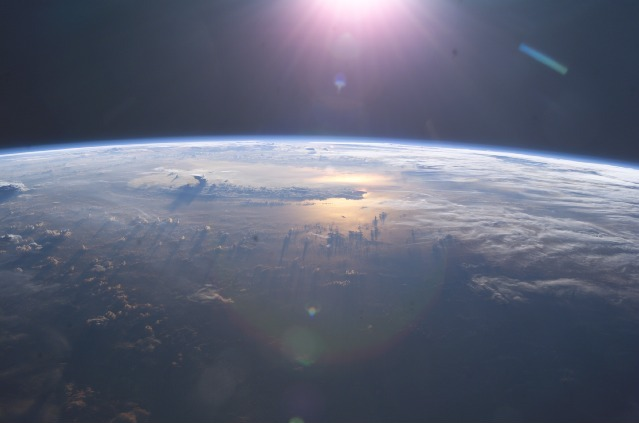
\includegraphics[width=0.35\paperwidth]{Images/Earth.jpg}};
\end{pgfonlayer}
%
\begin{pgfonlayer}{pic2}
\node[inner sep=0.5pt] (b) at (2.9,2.1)[draw=DarkGrey] {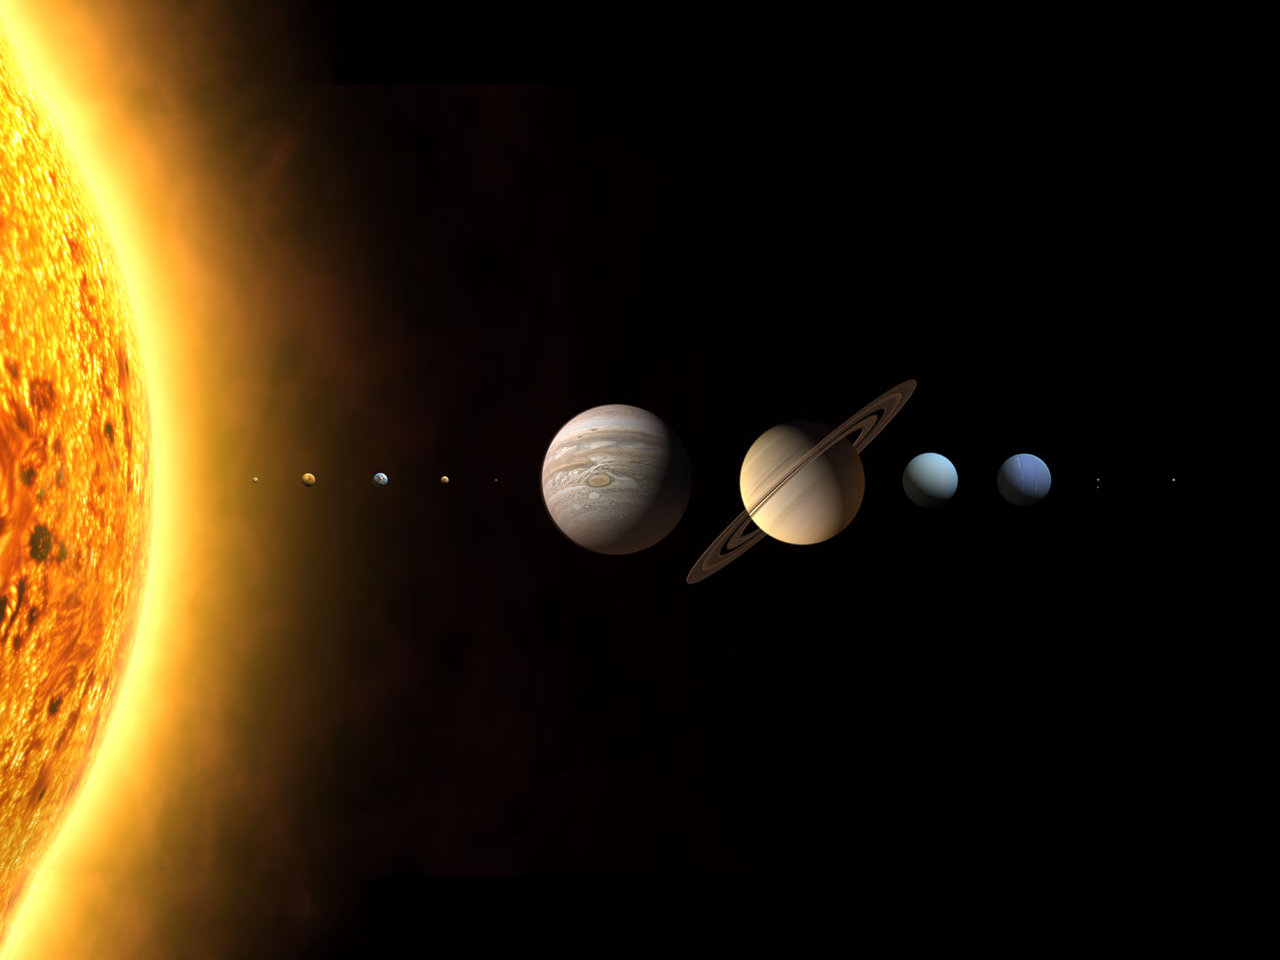
\includegraphics[width=0.35\paperwidth]{Images/solar_system1.jpg}};
\end{pgfonlayer}
%
\begin{pgfonlayer}{pic3}
\node[inner sep=0.5pt] (c) at (2.9,0.9)[draw=DarkGrey] {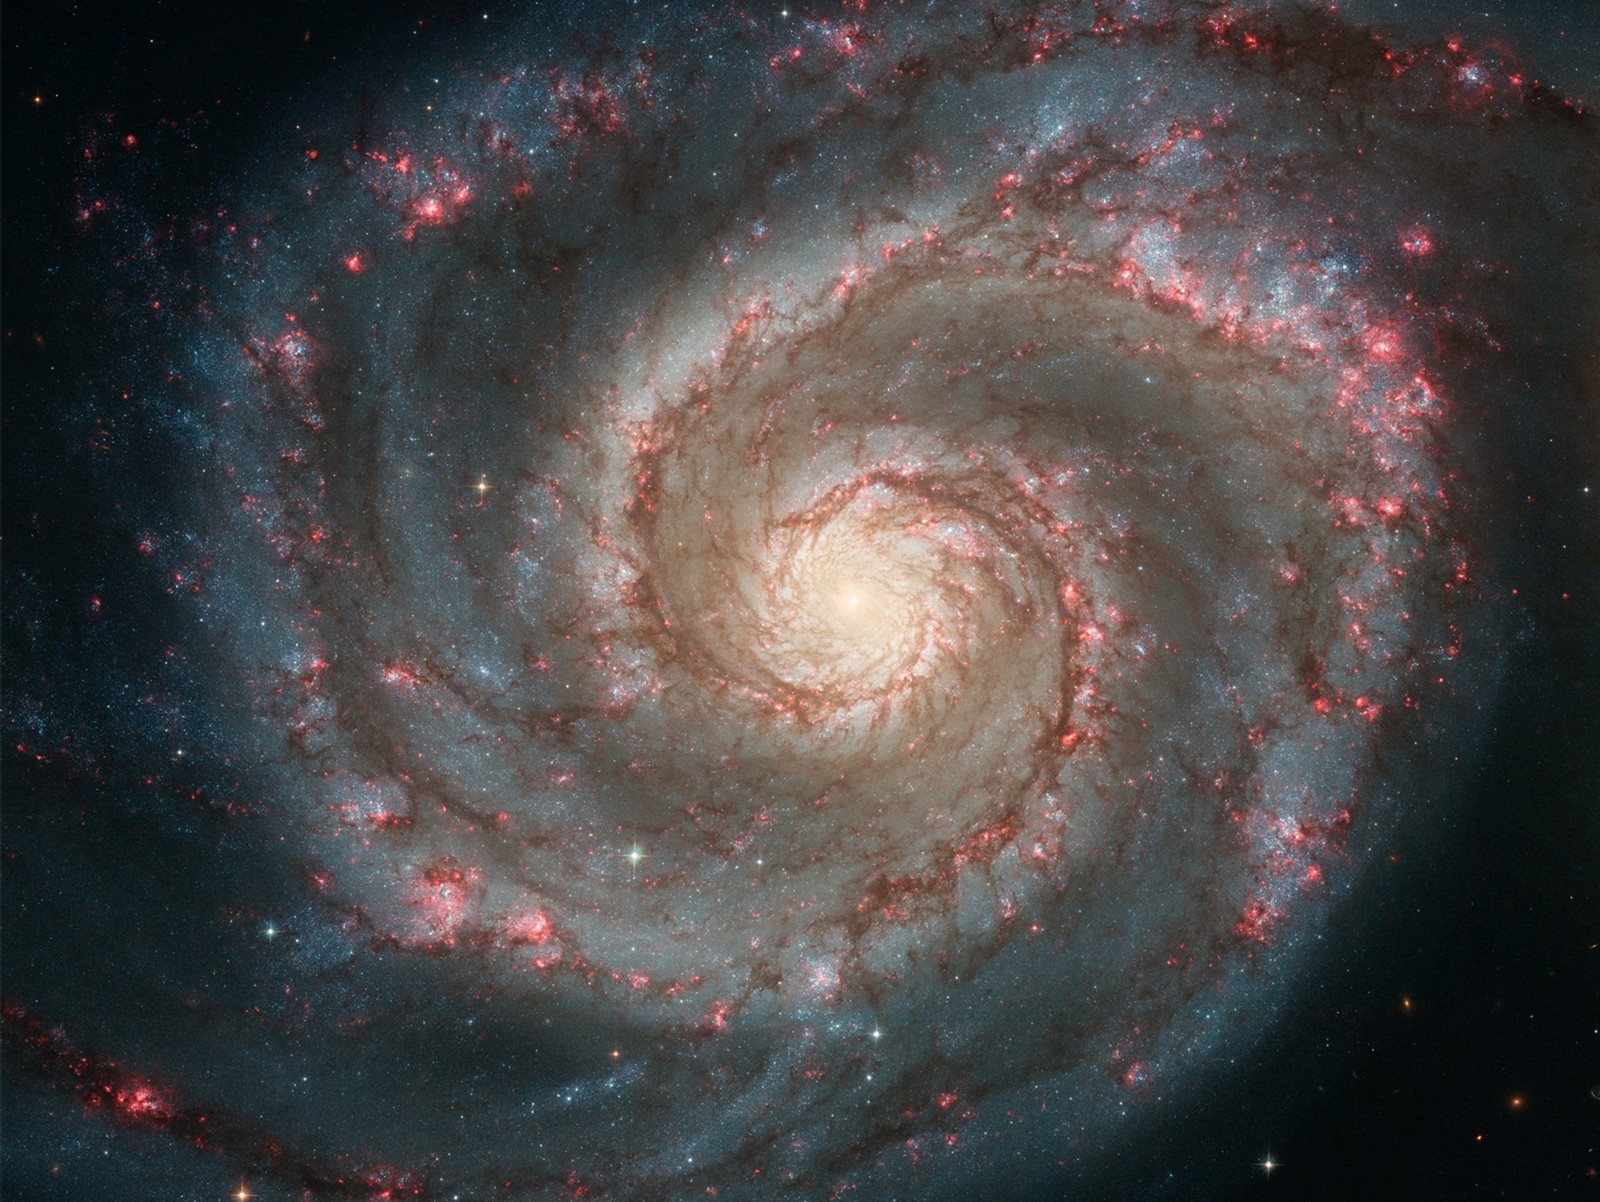
\includegraphics[width=0.35\paperwidth]{Images/milky_way.jpg}};
\end{pgfonlayer}
%
\begin{pgfonlayer}{pic4}
\node[inner sep=0.5pt] (d) at (1.1,0.9)[draw=red] {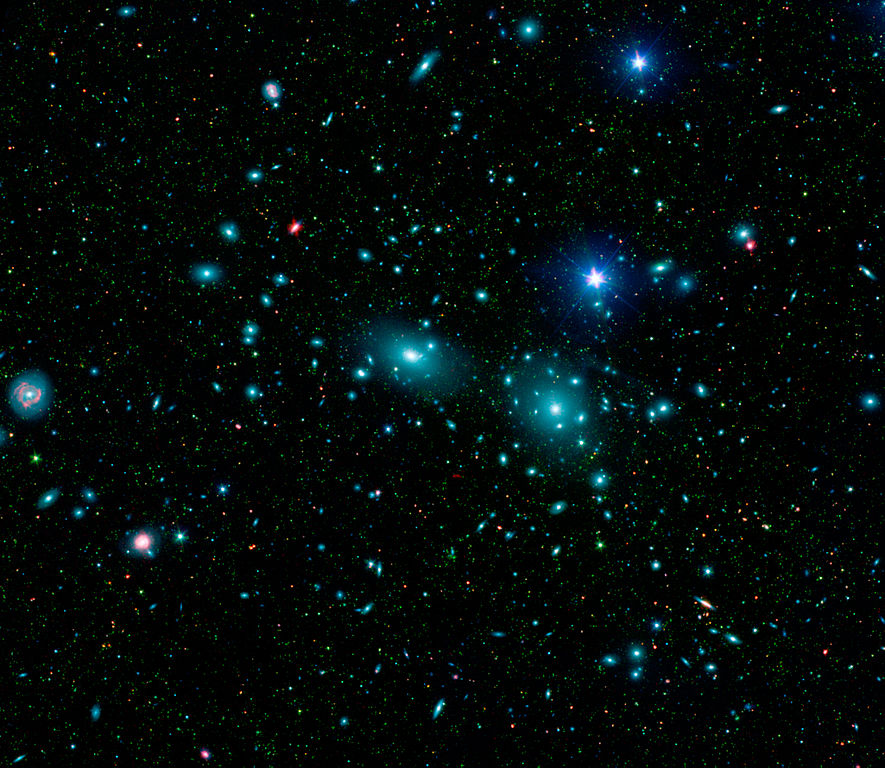
\includegraphics[width=0.35\paperwidth]{Images/Coma.jpg}};
\end{pgfonlayer}
}


\begin{frameb}{w}{Images/Coma.jpg}
	\frametitle{Galaxy Clusters}
	\begin{textblock}{20}(7,7)
	$\sim 10$ Mpc $\sim 30$ million light years
	\end{textblock}
\end{frameb}

\hierarchyblank
\hierarchy{
\begin{pgfonlayer}{pic1}
\node[inner sep=0.5pt] (a) at (1.1,2.1)[draw=DarkGrey] {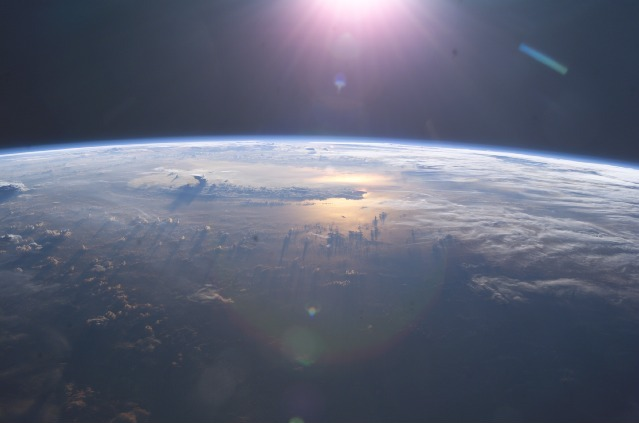
\includegraphics[width=0.35\paperwidth]{Images/Earth.jpg}};
\end{pgfonlayer}
%
\begin{pgfonlayer}{pic2}
\node[inner sep=0.5pt] (b) at (2.9,2.1)[draw=DarkGrey] {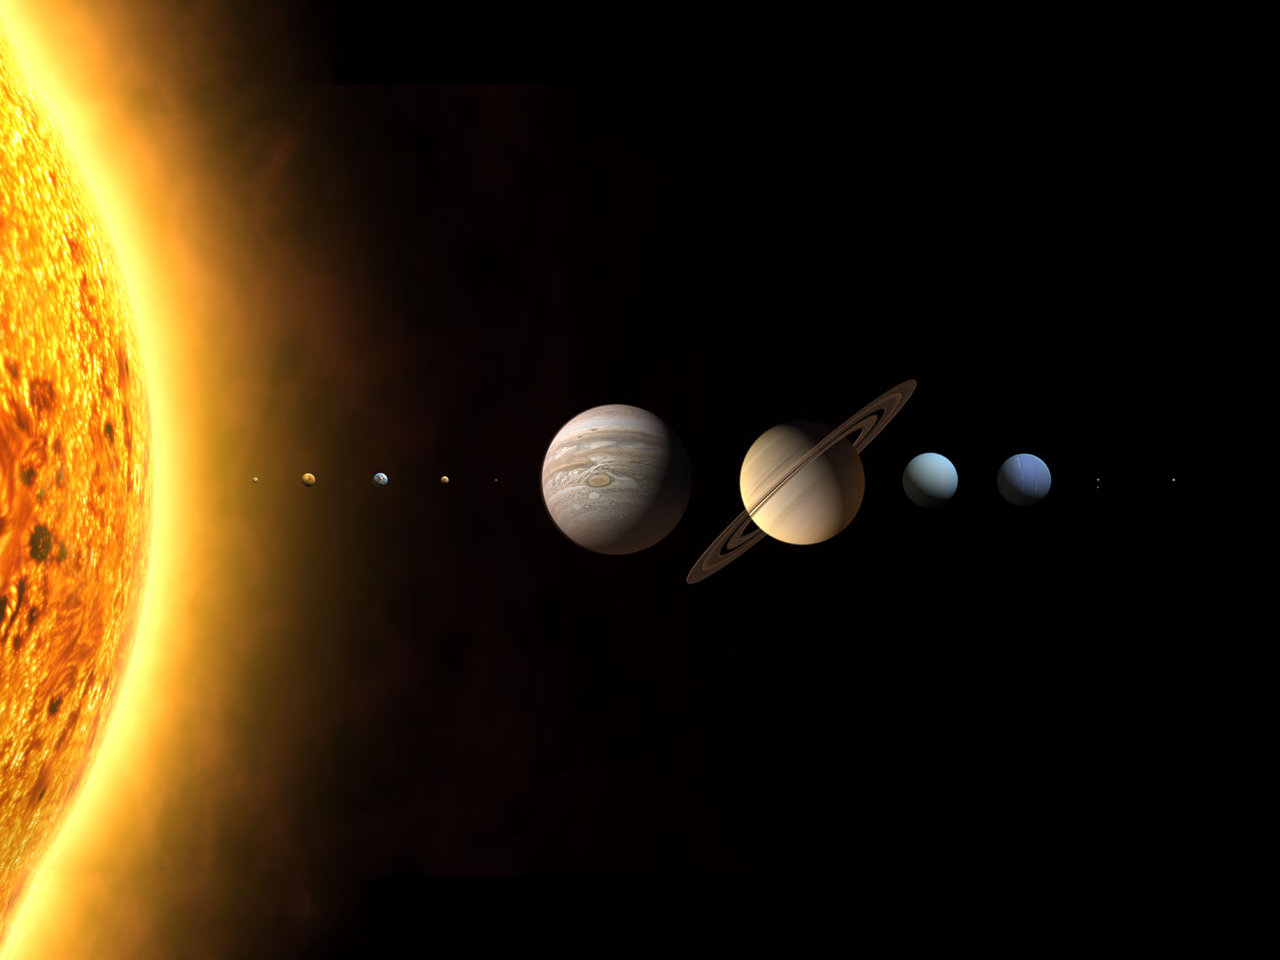
\includegraphics[width=0.35\paperwidth]{Images/solar_system1.jpg}};
\end{pgfonlayer}
%
\begin{pgfonlayer}{pic3}
\node[inner sep=0.5pt] (c) at (2.9,0.9)[draw=DarkGrey] {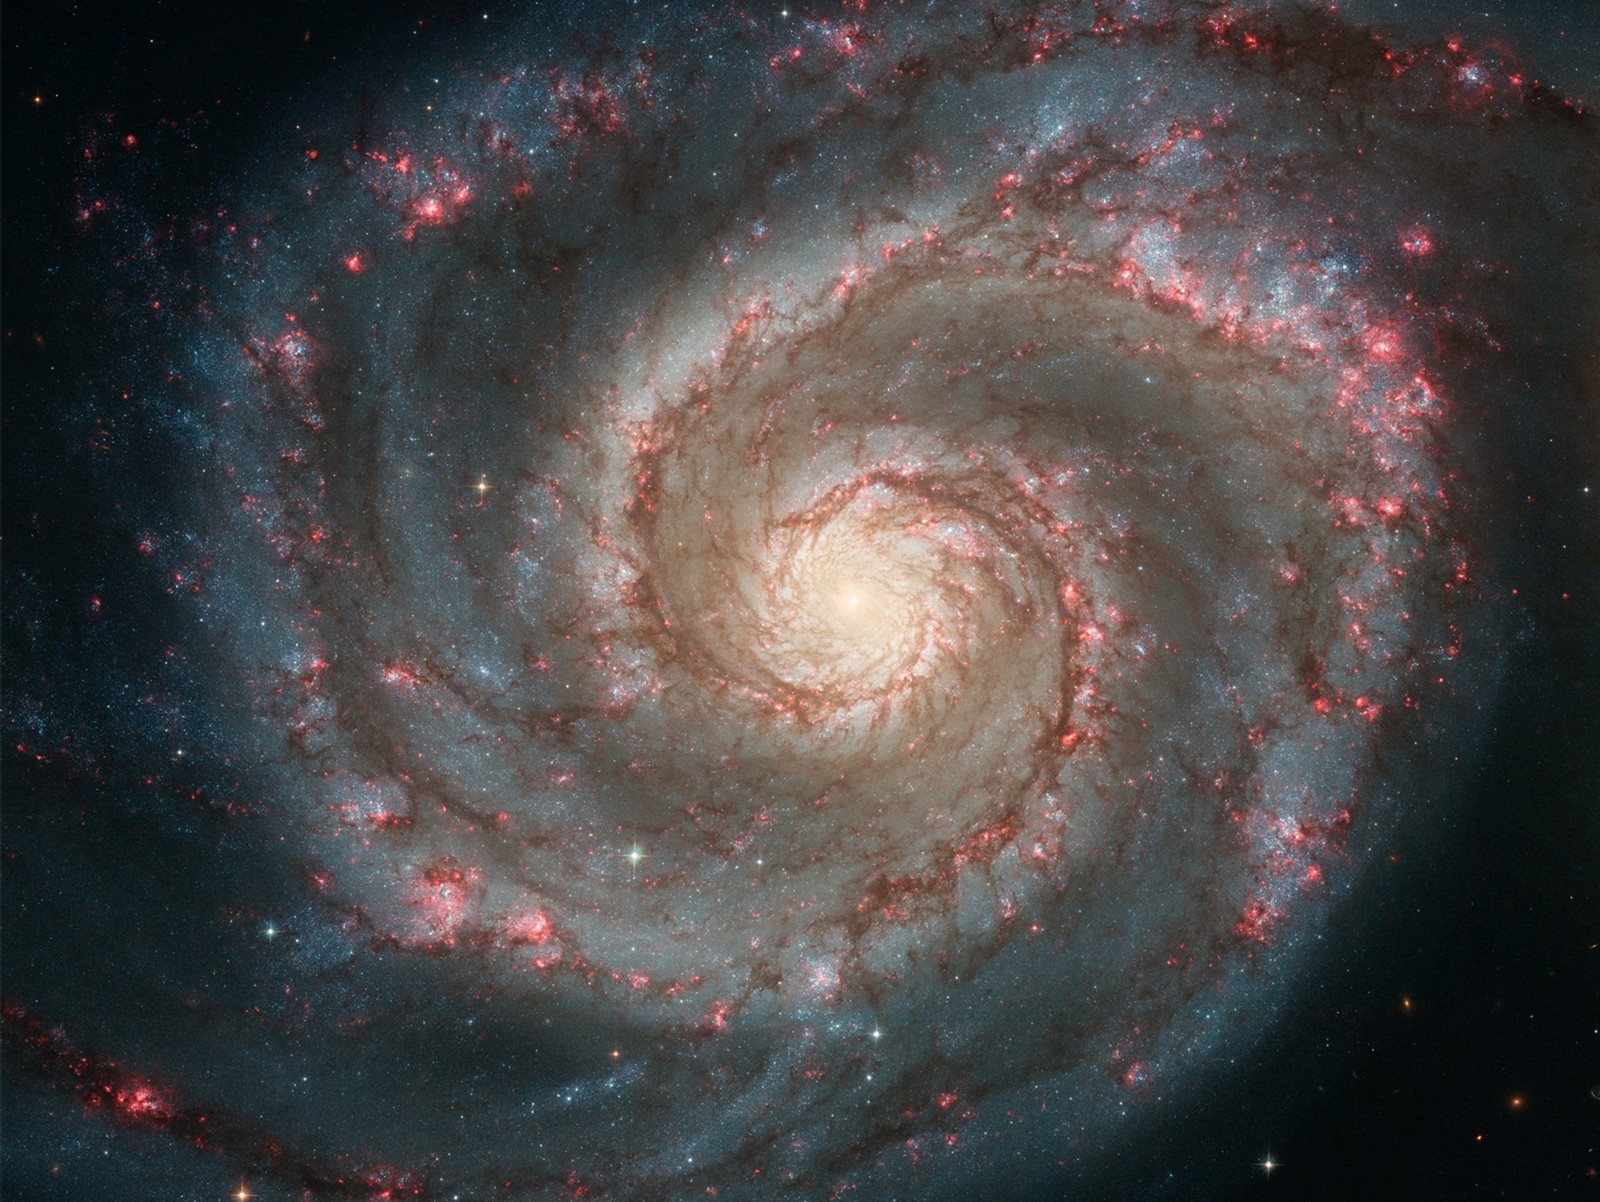
\includegraphics[width=0.35\paperwidth]{Images/milky_way.jpg}};
\end{pgfonlayer}
%
\begin{pgfonlayer}{pic4}
\node[inner sep=0.5pt] (d) at (1.1,0.9)[draw=DarkGrey] {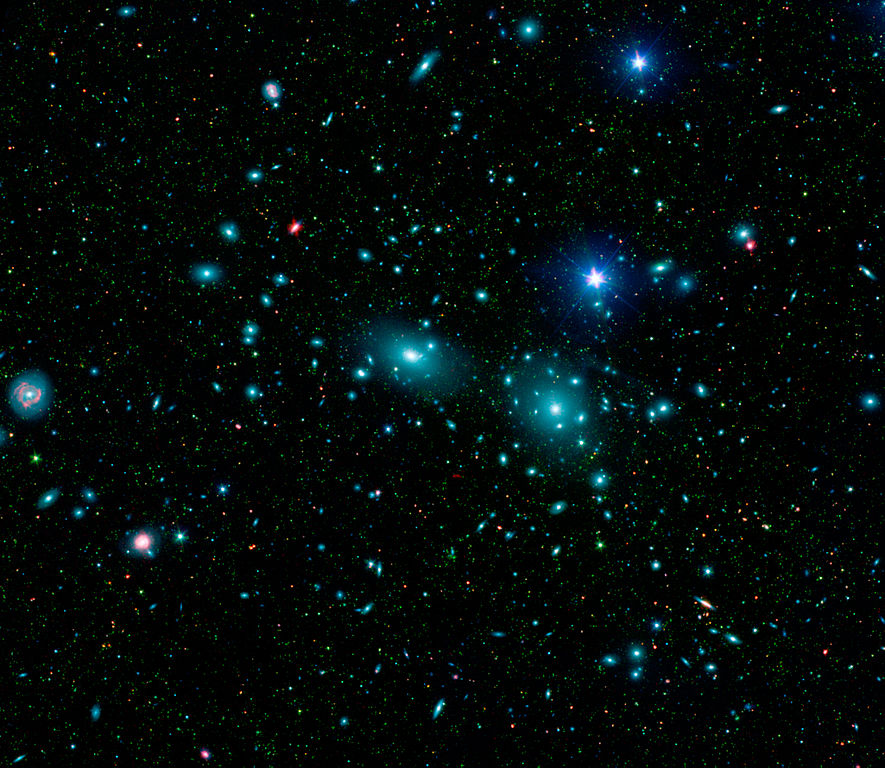
\includegraphics[width=0.35\paperwidth]{Images/Coma.jpg}};
\end{pgfonlayer}

\draw[draw=red,line width=2pt] (0,0.015) rectangle (3.985,3);
}

\begin{frameb}{w}{Images/XDF.jpg}
	\frametitle{Galaxy Clusters}
	\framesubtitle{Hubble extreme deep field}
\end{frameb}
